%------------------- Belt, Tensioner and Pulleys -------------------%
\subsection{Belt, Tensioner and Pulleys} \label{subsec:belt}

%------------------------------ Inputs and Outputs ------------------------------%
\subsubsection{Inputs and Outputs}

The main input for the belt design is the maximum moment generated at the knee joint $M_{max} = M_{knee} = 30.71 \text{ Nm}$ obtained from Figure \ref{fig:mod_torque_cycle} in Section \ref{sec:stability}.
Other inputs are the length of the thigh limb (from knee shaft to hip shaft) $L_{thigh} = 100 \text{ mm}$ and the distance between the hip motor shaft and the knee motor shaft $L_{hm2km} = 88 \text{ mm}$ which form the center distance $C$. 
\begin{equation}
    C = L_{thigh} + L_{hm2km} = 100\text{ mm} + 88\text{ mm} = 188\text{ mm}
\end{equation}

The outputs are the belt's tight tension $T_{tight}$ and slack tension $T_{slack}$, the pulleys' pitch diameter $D_{pitch}$, outer overall diameter $D_O$ including the belt, number of teeth $N_{pulley\  teeth}$, the belt's length $L_{belt}$ and number of teeth $N_{belt\ teeth}$ along with other dimensions for the CAD model.

%------------------------------ CONSTANTS ------------------------------%
\subsubsection{Constants and Parameters}

The mechanical efficiency of the belt is known to be somewhere between 94\% and 96\% \cite{gates_mectrol_timing_2006}. A value of $\eta_{belt} = 0.95$ was chosen for this application. The chosen belt has a constant tooth pitch $p$ of 8 mm per tooth and a width $w$ of 25 mm. The pulleys' number of teeth $n_{teeth}$ is a variable parameter that will change based on the maximum torque at the knee joint, but the value chosen for the calculations is 21 teeth for both pulleys. The pitch diameter of the pulley can be calculated as follows \cite{gates_mectrol_timing_2006}:
\begin{equation}
    D_p = \frac{p\ n_{teeth}}{\pi} = \frac{(8\text{ mm/tooth})\ (21 \text{ teeth})}{\pi} = 53.48\text{ mm}
\end{equation}
%------------------------------ Assumptions ------------------------------%
\subsubsection{Assumptions and Simplifications}

It is assumed that both pulleys have the same diameter ($D_{hip} = D_{knee} = 53.48\text{ mm}$) since no further speed reduction is required. This also simplifies the design calculations. The impact of gravity and inertia of both pulleys and the belt were neglected due to the low velocity and acceleration of the limbs. \\

%------------------------------ Materials ------------------------------%
\subsubsection{Material Selection}

The chosen timing belt manufacturer, Gates Mectrol, offers urethane belts reinforced with either steel or Kevlar. Both products offered different limits when it comes to the maximum tension that can be applied on a belt. However, since the steel reinforced belts are able to take higher loads than the Kevlar ones, steel was chosen to minimize the size of both the belt and the pulleys \cite{gates_mectrol_urethane_2018}. The chosen belt, a steel reinforced HTD\textsuperscript{\textregistered}8 urethane timing belt has a maximum allowable belt tension $T_{max}$ of $3471\text{ N/}25\text{ mm}$ of belt width as shown in the Gates Mectrol Urethane Belt Catalogue on page 9 in Appendix \ref{app:datasheets} \cite{gates_mectrol_urethane_2018}. The manufacturer also suggests an allowable effective tension $T_{e\ allow}$ of $1870 \text{ N/}25\text{ mm}$ of belt width that is valid only if 15 teeth or more are used for meshing. This condition means that the allowable effective tension value given only applies if the the two pulleys have at least 30 teeth and therefore cannot be used for this present case.

As for the pulleys, Gates Mectrol offers aluminium, steel, and stainless steel as options for the pulley material \cite{gates_mectrol_urethane_2018}. Zinc plated steel or stainless steel flanges may also be added to the pulley to help maintain the position of the belt. The chosen material is aluminium since both pulleys are sealed from the environment, and because a reduced weight has a positive effect on the robot's general capabilities.

%------------------------------ Free-Body Diagram ------------------------------%
\subsubsection{Free-Body Diagram}

The free-body diagrams of both pulleys are presented in Figure \ref{fig:KneePulley} and Figure \ref{fig:HipPulley}.

\begin{figure}
    \centering
    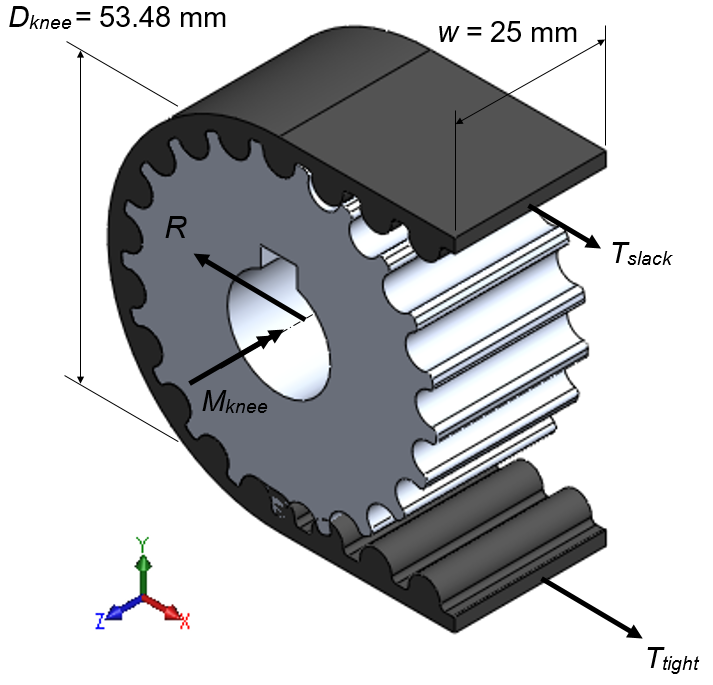
\includegraphics[width=0.5\textwidth]{4_Analysis/img/Belt/Knee_Pulley_Ann.PNG}
    \caption{Knee pulley FBD}
    \label{fig:KneePulley}
\end{figure}
\begin{figure}
    \centering
    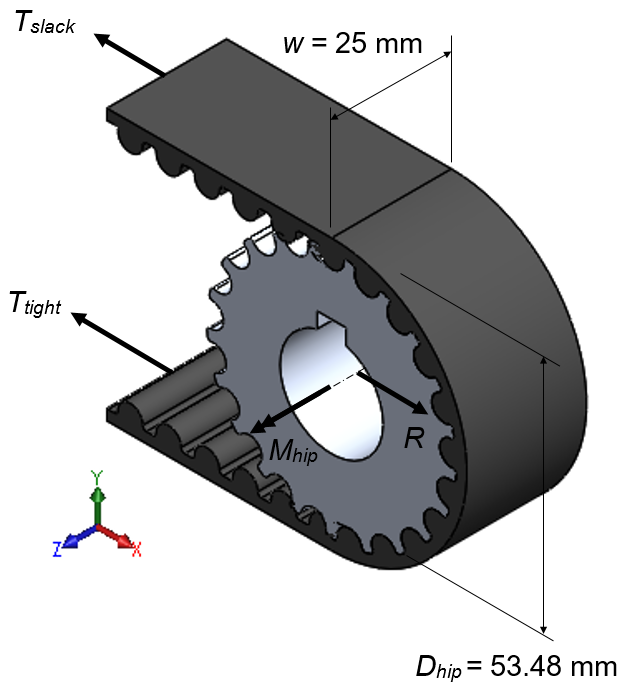
\includegraphics[width=0.5\textwidth]{4_Analysis/img/Belt/Hip_Pulley_Ann.PNG}
    \caption{Hip pulley FBD}
    \label{fig:HipPulley}
\end{figure}
%------------------------------ Stress Analysis ------------------------------%
\subsubsection{Stress Analysis}

The moment taken by the driving pulley is expressed as follows \cite{gates_mectrol_timing_2006}.
\begin{equation}
    M_{hip} = \frac{M_{knee}}{\eta_{belt}}\frac{D_{hip}}{D_{knee}} = \left(\frac{30.71 \text{ Nm}}{0.95}\right)\left(\frac{53.48\text{ mm}}{53.48\text{ mm}}\right) = 32.26 \text{ Nm}
\end{equation}
Then, the effective tension of the belt $T_e$ can be obtained from the driving torque.
\begin{equation}
    T_e = \frac{2M_{hip}}{D_{hip}} = \frac{2(32.36 \text{ Nm})}{53.48 \text{ mm}\ \frac{1\text{ m}}{1000\text{ mm}}} = 1209\text{ N}  
\end{equation}
The effective tension of the belt can also be expressed by the difference between the tight tension and the slack tension and timing belts are known to perform better when the slack tension is 10\% to 30\% the magnitude of the effective tension \cite{gates_mectrol_timing_2006}. 30\% was chosen as a conservative approach for increasing the load on the belt.
\begin{equation}
    T_{slack} = 0.3 \ T_e = (0.3)\ 1209 \text{ N} = 362.7 \text{ N}
\end{equation}
Then, the tight tension can be obtained as follows.
\begin{equation}
    T_{tight} = T_e + T_{slack} = 1209\text{ N} + 362.7\text{ N} = 1571.7\text{ N}
\end{equation}
The tight and slack tensions can be added to obtain the resultant reactive force on either shaft.
\begin{equation}
    \sum F_x = 0 \longrightarrow R = T_{tight} + T_{slack} = 1571.7\text{ N} + 362.7\text{ N} = 1934.4\text{ N}
\end{equation}

Now, to compare the belt tensions with the manufacturer's recommendations to obtain safety factors.
\begin{equation}
    SF = \frac{T_{max}}{T_{tight}} = \frac{3741\text{ N}}{1571.7\text{ N}} = 2.38
\end{equation}
\begin{equation}
    SF^* = \frac{T_{e\ allow}}{T_e} = \frac{1870\text{ N}}{1209\text{ N}} = 1.55
\end{equation}
However, $SF^*$ may not mean anything since the condition of minimum 15 teeth in meshing is not respected for two pulleys with 21 teeth each.\\

The total length of the belt $L_{belt}$ and the number of teeth $N_{teeth}$ can be obtained as follows \cite{gates_mectrol_timing_2006}.
\begin{equation}
    L_{belt} = 2C + \pi D_p = 2(188\text{ mm}) + \pi(53.48\text{ mm}) = 544\text{ mm}
\end{equation}
\begin{equation}
    N_{teeth} = \frac{L_{belt}}{p} = \frac{544\text{ mm}}{8\text{ mm/tooth}} = 68\text{ teeth}
\end{equation}

%------------------------------ Critical Review ------------------------------%
\subsubsection{Critical Review}
The pulley dimensions obtained above are sufficient to reduce the belt tensions to acceptable values based on the manufacturer's recommendations. An error may have been made when the efficiency of the belt was applied: for a case where the motor is not powered, the driver pulley actually becomes the knee pulley and the motor shaft is then driven. Therefore, the torque on the motor shaft should be lower than torque on the knee pulley. However, wrongfully applying the efficiency of the belt drive only makes this analysis more conservative and has no negative effects on the results. This error may be corrected for the parameterization. \\

The analysis of the torsion spring belt tensioner was attempted but did not yield satisfying results. No direct link could have been made between the belt tension and the properties of the torsion spring. It was then decided that the belt's total length $L_{belt}$ would tightly fit the over the pulleys when installed by hand. Then, the installation of the torsion spring only helps ensuring that the belt tension remains in an operating range if the belt were to expand due to the temperature or due to normal life wear. The spring dimensions were chosen following a similar process as the other torsion springs in Section \ref{subsec:Tspring} but no further analysis was completed. The main spring dimensions are as follows: free angle $\beta = 270^{\circ}$, wire diameter $d = 2\text{ mm}$, coil diameter $D = 10\text{ mm}$, arm length $l = 24\text{ mm}$, number of body turns $N_b = 14.75\text{ turns}$. The spring constant $k$ was found to be $327.3\text{ Nmm/rad}$, the maximum deflection $\theta_{max}$ is approximately $155^{\circ}$ which yields a maximum torque $M_{max}$ of $885.44\text{ Nmm}$ while respecting a safety factor of 1.03 if the belt were to perfectly straighten as shown on Figure \ref{fig:beltTight} in the Detailed Design Section. If a single tensioner is not sufficient for the continuous operation of the robot, an identical torsion spring could be added on the other side of the belt to compensate for the bidirectional drive.

%------------------------------ Parameterization ------------------------------%
\subsubsection{Parameterization}
The idea behind the parameterization of this analysis consists of inputting the highest torque generated at the knee and the distance between the input and output shafts to obtain the pulley and belt dimensions. A loop will most likely be used to obtain an optimized value for the pulley diameter based on the tensile limits of the belt and the other belt dimensions that will remain constant. The tensioner will most likely not be parameterized due to the constant belt width and belt pitch.